\chapter{Boosted Decision Trees}
\label{chap:bdt}

This chapter descibes the boosted decision tree algorithm and its use
in the VBF \hwwlnln analysis.

\section{What is a boosted decision tree?}

Boosted decision trees (BDTs) fall into a class of algorithms called machine learning
algorithms. In these algorithms, a computer constructs a model of the
relationship between independent variables (features) and some
dependent variable in a process called training. These algorithms can
be used for classification of objects that fall into different classes
(ie, signal vs. background) or for regression in the case of a
continuously-distributed, real-valued dependent variable. Machine
learning, and in particular decision trees, are increasingly used in
particle physics for particle identification and event
classification (references). At the LHC, BDTs have been used by both
CMS and ATLAS (references). 

A decision tree is a sequence of selection cuts on the independent
variables, which is shown schematically in
Fig~\ref{chap:bdt:fig:bdt_schem}. In order to grow a decision tree, a
training set of events representing the two classes (signal and
background) is used. In the case of the VBF analysis, fully simulated
Monte Carlo samples are used for both signal and background. Starting
at the root node, the algorithm loops through the independent
variables, finding the one that best separates signal and
background. The separation is quantified by the Gini index, given by
$p(1-p)$, where p is the signal purity $\frac{S}{S+B}$. A cut is
placed on the independent variable yielding the minimum Gini index,
splitting the training sample into two orthogonal subsets. The
procedure is then repeated at the two nodes representing the first
decision tree layer, yielding two more cuts and a total of four
sub-samples. The process is repeated until a minimum number of events
per node or maximum tree depth is reached. The final nodes, called
leaves, are assigned a value of -1 if the majority of the events are
background and a value of 1 if the majority of the events are signal. 

The discriminating power of a decision tree classifier lies in its ability to take advantage of
the correlations among the independent variables. To illustrate this,
consider a toy example in which there are two variables, $x_1$ and
$x_2$, plotted in for signal and background in
Figure~\ref{chap:bdt:fig:x1_x2}, where the high degree of
correlation is visible. Performing a cut optimization on the two input
distributions, and choosing a signal acceptance working point of
50$\%$ results in the selected box shown in
Figure~\ref{chap:bdt:fig:x1_x2} (a). Because a decision tree is a
sequence of binary cuts, it can be conceptualized as a collection of
boxes in phase space. If the correlations between input variables are
different for signal and background, as is the case for the toy
example, then the decision tree can partition the phase space into
several signal-rich regions, thereby enhancing the separation
power. This is shown in Figure~\ref{chap:bdt:fig:x1_x2} (b), where the
decision tree picks out a second signal-rich region. Setting the
signal acceptance to the same working point, the decision tree results
in a signal purity, $frac{S}{S+B}$, of 92$\%$, while the signal purity
with square cuts is 82$\%$.

In general for classification problems, it is uncommon to use a single
decision tree

\begin{figure}[h]
    \centering
    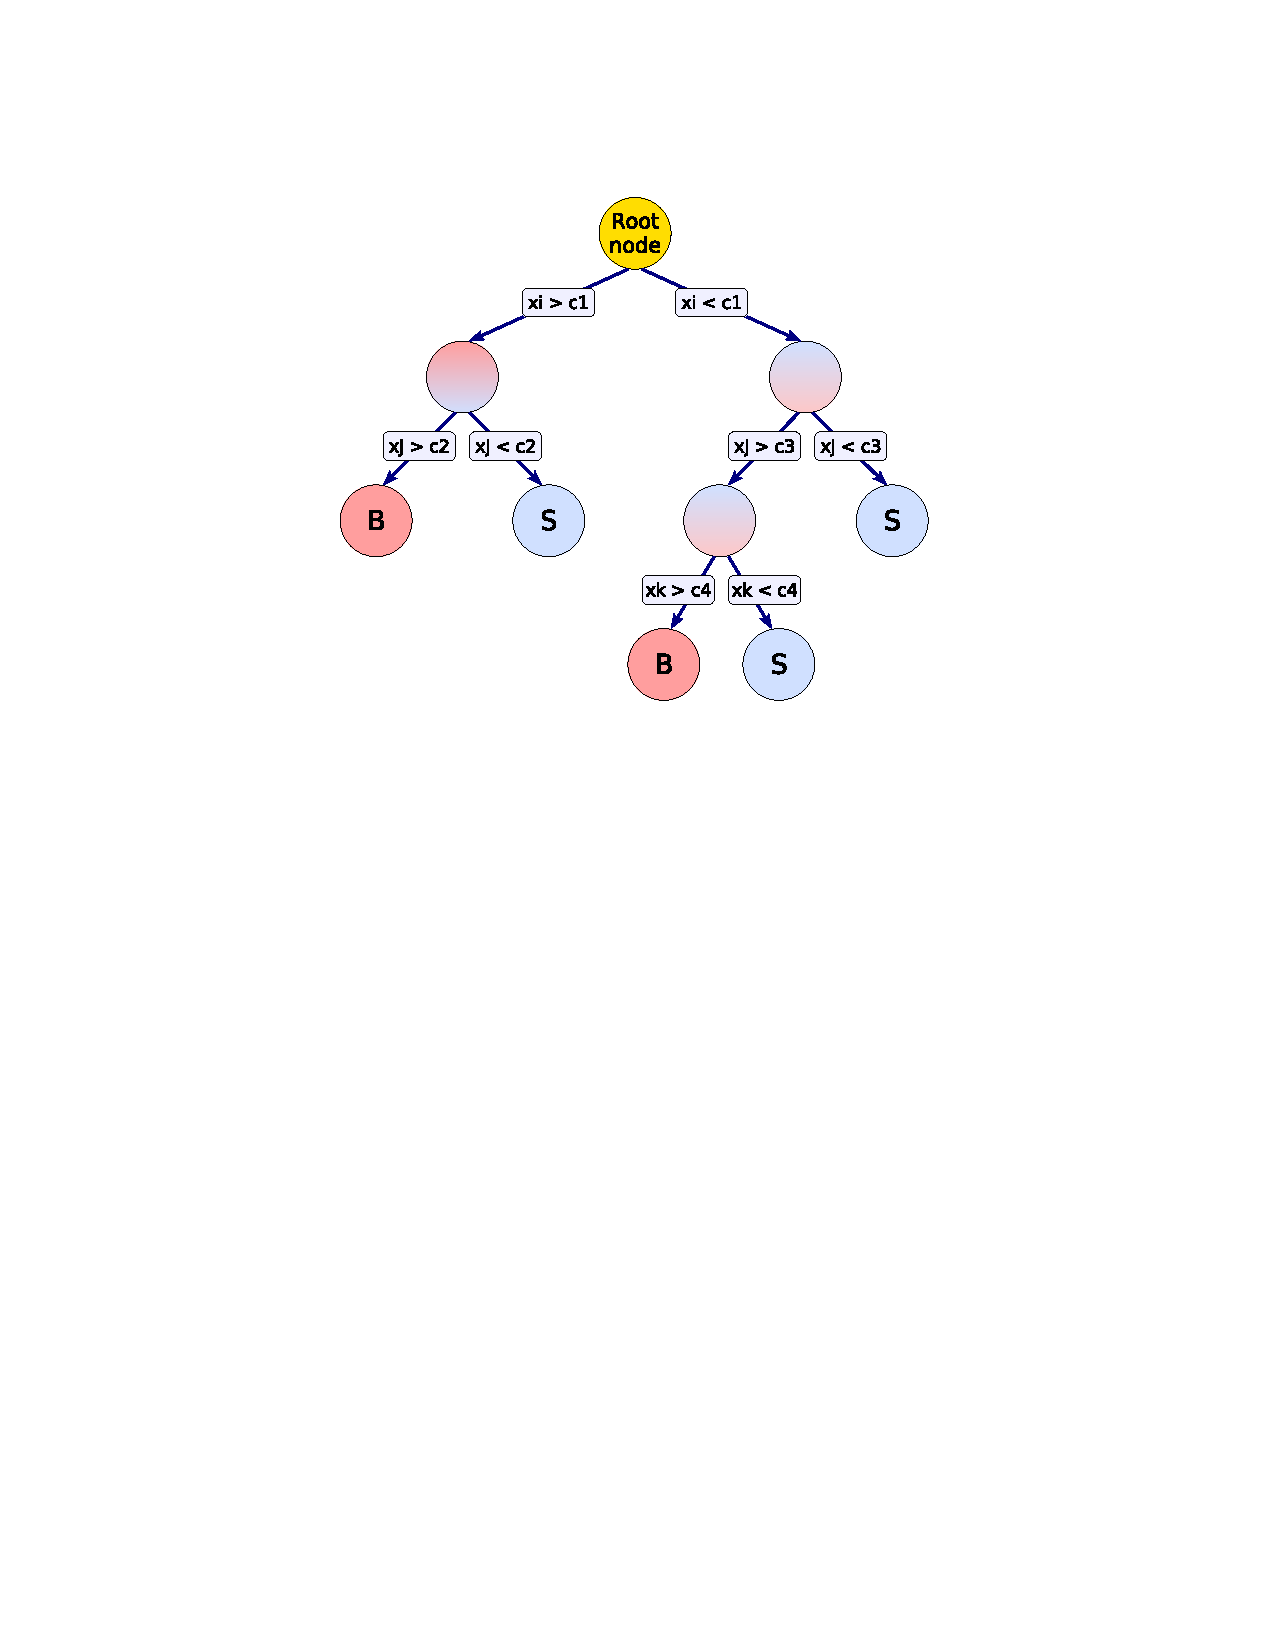
\includegraphics[width=0.90\textwidth]{bdt/bdt_schematic.pdf}
    \caption[Schematic of a boosted decision tree.~\cite{bib:Therhaag:2009dp}].
\label{chap:bdt:fig:bdt_schem}
\end{figure}

\begin{figure}[h]
    \centering
    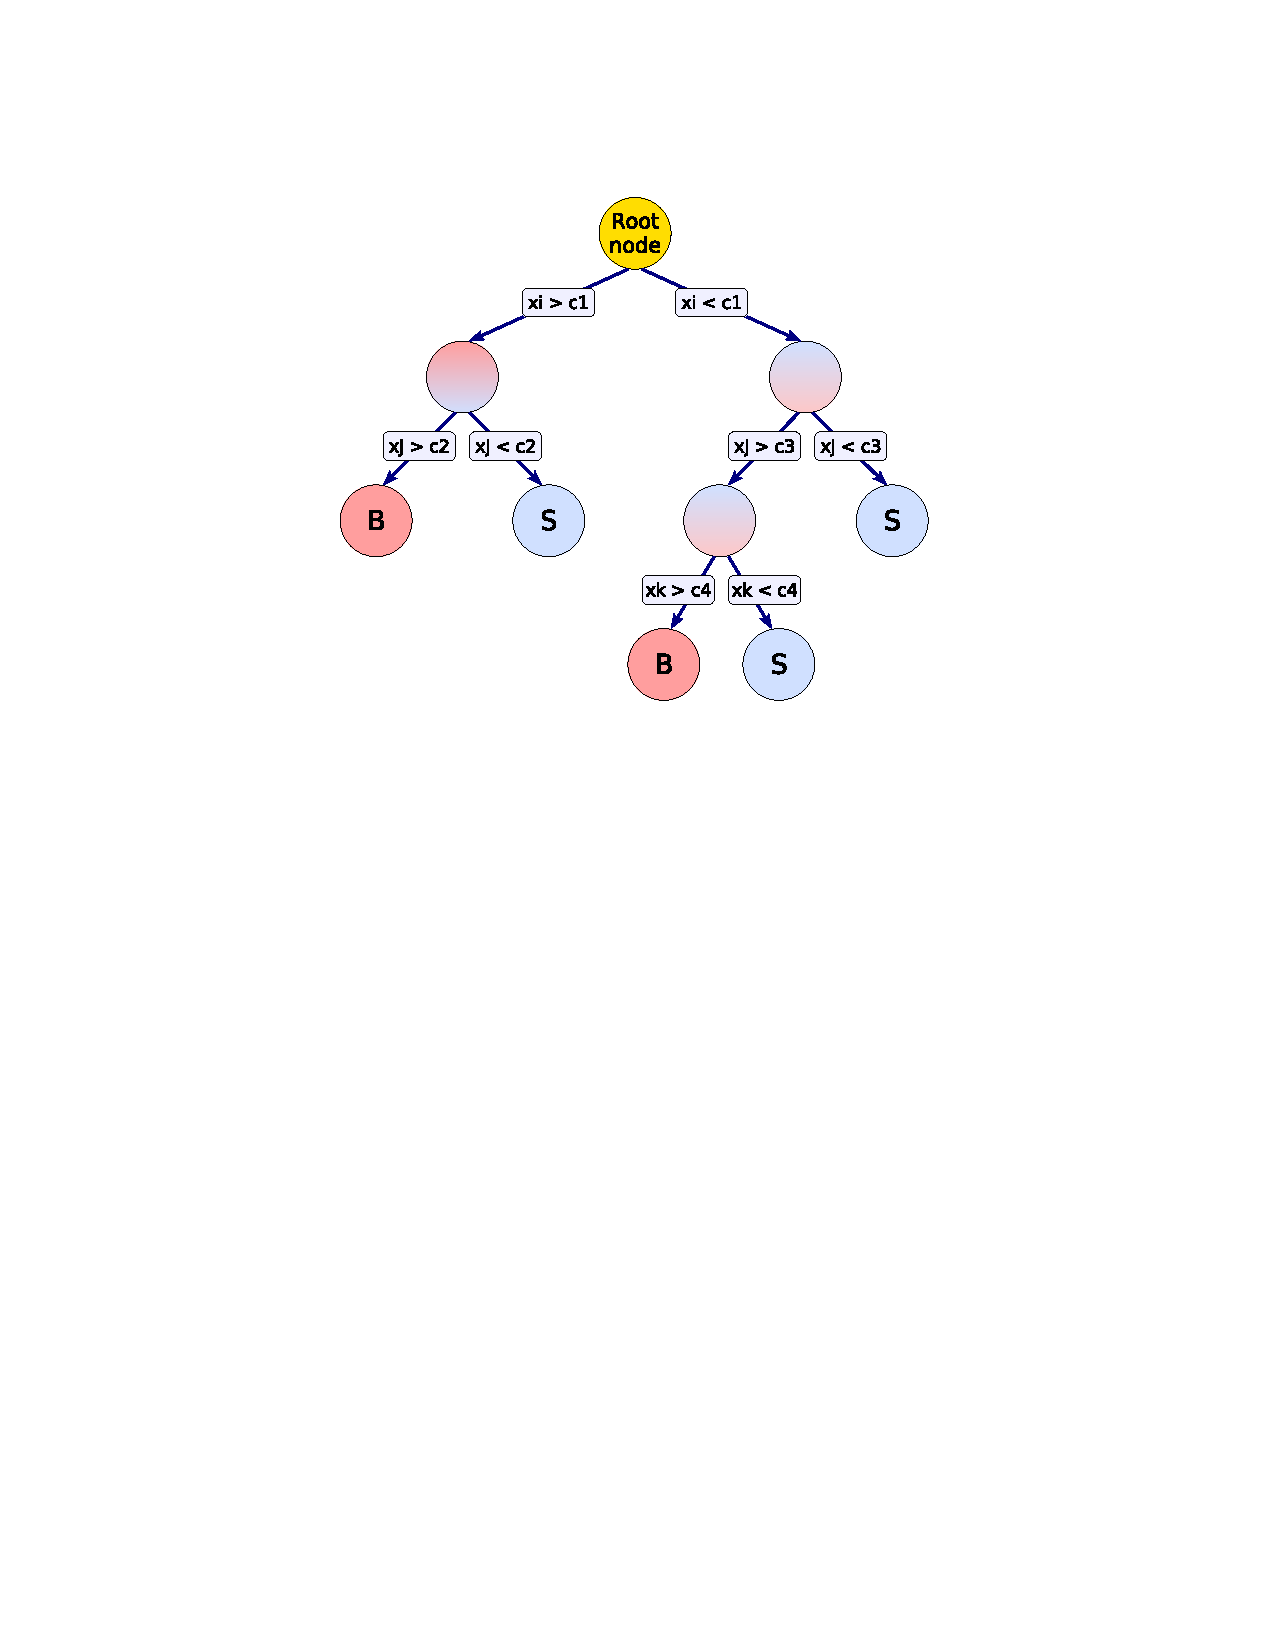
\includegraphics[width=0.90\textwidth]{bdt/bdt_schematic.pdf}
    \caption[Schematic of a boosted decision tree.~\cite{bib:Therhaag:2009dp}].
\label{chap:bdt:fig:x1_x2}
\end{figure}
